\documentclass[
version=last,toc=bib,toc=graduated,toc=index,toc=listof,9pt,openany]{scrbook}
%\pdfminorversion=4
\usepackage{polyglossia}
\setdefaultlanguage{english}

\setmainfont{Source Sans Pro}
\setsansfont{Source Sans Pro}

\usepackage{ifmtarg}
\usepackage{ifthen}
\usepackage{etoolbox} % \ifstrempty

\usepackage{geometry}
\geometry{%a6paper
paperwidth=125mm, paperheight=168mm, 
portrait,
top=22mm,
inner=22mm,
outer=20mm,
bottom=25mm,
headsep=3mm,
footskip=12mm
}

\usepackage{ragged2e} % nicer typesetting (hyphenation) for non raggedright and raggedleft
\usepackage{lscape}
\setlength{\parskip}{0pt}

\usepackage{relsize}

\clubpenalty=10000
\widowpenalty=10000 
\displaywidowpenalty=10000

\usepackage[]{microtype}

\usepackage{graphicx} % graphics

% search path for images
\graphicspath{{images-print/}{icons/}{extra-pages/}{wallpaper/}}
\usepackage{wrapfig}  % sponsor logos wrapped with text

\usepackage{tabu}
\usepackage{tabularx}
\usepackage{longtable}
\usepackage[table,cymk]{xcolor}
\usepackage{colortbl}

% embed PDF pages
% pdfpages must not be loaded before colortbl!
\usepackage{pdfpages}
% TikZ must not be loaded before colortbl
\usepackage{tikz}

\usepackage{multirow}
\usepackage{booktabs}
\usepackage{array}

% multiple text columns (list of thanks)
\usepackage{multicol}

\usepackage{refcount} % calculation of the page where the map is located

% page background
\usepackage[manualmark]{scrlayer-scrpage}
\pagestyle{scrplain}

\newcommand{\acro}[1]{{\textsmaller{#1}}} % macro for abbreviations with more than one capitalised letter


% title/metadata
\title{State of the Map 2018}
\subtitle{Programme}
\author{OpenStreetMap Foundation}
\date{\today}

\clearscrheadings

% page numbers
\cfoot[\begin{small}\pagemark\end{small}]{\begin{small}\pagemark\end{small}}
\ofoot[]{}
\ifoot[]{}
\pagestyle{scrplain}

\linespread{1.15}

% include our custom macros
\input{abstract-commands}
% OSMF
\DeclareNewLayer[background,%
  width=125mm,%
  height=168mm,%
  contents={%
    \includegraphics{wallpaper/osmf.pdf}%
  }%
]{osmfmap}
\newpairofpagestyles{osmf}{}
\AddLayersAtBeginOfPageStyle{osmf}{osmfmap}

% metro map of Milan
\DeclareNewLayer[background,%
  width=125mm,%
  height=168mm,%
  contents={%
    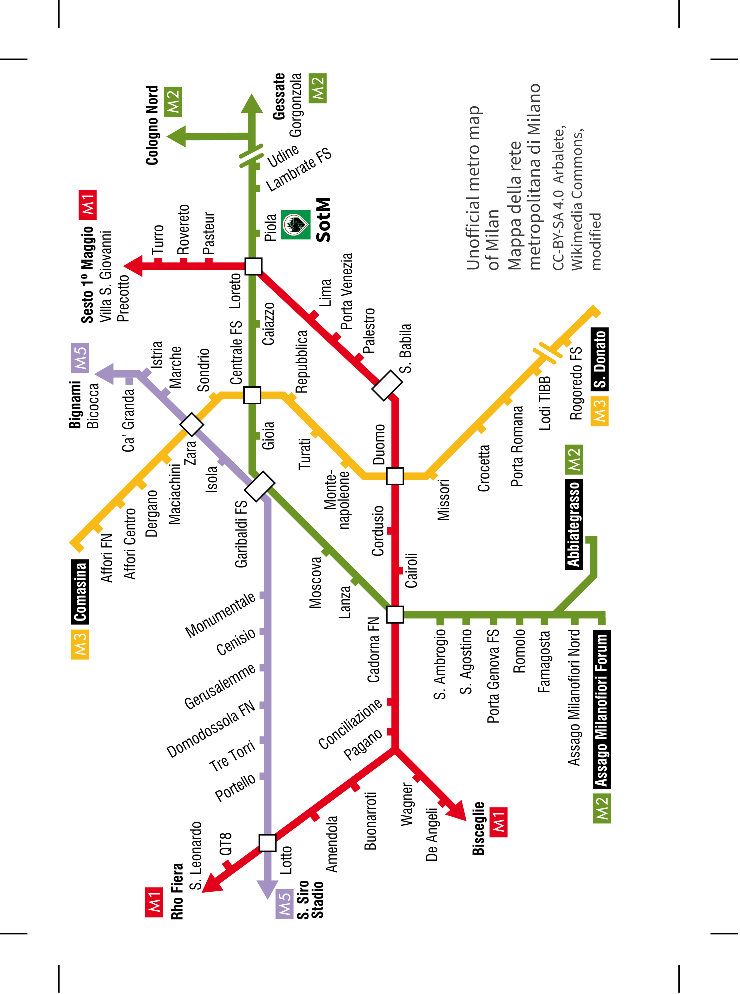
\includegraphics{wallpaper/metro.pdf}%
  }%
]{metromap}
\newpairofpagestyles{metro}{}
\AddLayersAtBeginOfPageStyle{metro}{metromap}

% Microsoft advertisement
\DeclareNewLayer[background,%
  width=125mm,%
  height=168mm,%
  contents={%
    \includegraphics{sponsors/microsoft-cropped-compressed.pdf}%
  }%
]{microsoftadvertisement}
\newpairofpagestyles{sponsor-microsoft}{}
\AddLayersAtBeginOfPageStyle{sponsor-microsoft}{microsoftadvertisement}

% Facebook advertisement
\DeclareNewLayer[background,%
  width=125mm,%
  height=168mm,%
  contents={%
    \includegraphics{sponsors/facebook.pdf}%
  }%
]{facebookadvertisement}
\newpairofpagestyles{sponsor-facebook}{}
\AddLayersAtBeginOfPageStyle{sponsor-facebook}{facebookadvertisement}

% Mapbox advertisement
\DeclareNewLayer[background,%
  width=125mm,%
  height=168mm,%
  contents={%
    \includegraphics{sponsors/mapbox.pdf}%
  }%
]{mapboxadvertisement}
\newpairofpagestyles{sponsor-mapbox}{}
\AddLayersAtBeginOfPageStyle{sponsor-mapbox}{mapboxadvertisement}

% Kaart/Maps.Me advertisement
\DeclareNewLayer[background,%
  width=125mm,%
  height=168mm,%
  contents={%
    
\includegraphics{sponsors/kaart-mapsme.pdf}%
  }%
]{kaartmapsmeadvertisement}
\newpairofpagestyles{sponsor-kaartmapsme}{}
\AddLayersAtBeginOfPageStyle{sponsor-kaartmapsme}{kaartmapsmeadvertisement}


\begin{document}
 
\pagestyle{cropmarksstyle}
\begin{titlepage}
  \thispagestyle{titlestyle}
  \null
\end{titlepage}
\pagestyle{cropmarksstyle}

\selectlanguage{english}
\input{contents}
\input{welcome}
\input{scholarships}
\section*{Getting around in Milan}
\label{getting-around}
\pagestyle{cropmarksstyle}
Azienda Trasporti Milanesi (ATM) operates a public transport network in Milan. Single tickets cost
€~1.50 and are available from newsstands, tobacconists (tabaccherie), bars and automatic ticket
machines in metro stations. 24\,h (€~4.50) and 48\,h (€~8.25) tickets, as well as a \emph{carnet} of 10 single
trips (€~13.80) are also available. An evening ticket (€~3.00) allows unlimited travel after 20:00.

Tickets should be stamped at the start of every journey and every time you change vehicles. To stamp
your ticket insert it into the slot in the electronic ticket machine on board overground vehicles or
at the ticket barriers in the metro. It is then valid for 90 minutes unlimited use (bus or tram), or
the completion of your full metro journey. Tickets are not sold on board and you will not find a
self-service ticket machine at bus and tram stop.

If your journey starts with the Metro, you can also use contactless payment.
Fees are limited so that you do not pay more than the 24 hr rate on any day.

\section*{Code of Conduct}
\label{coc}
The OSM Foundation is dedicated to providing a harassment-free
conference experience for everyone, regardless of gender, gender identity
and expression, sexual orientation, disability, physical appearance, body
size, race, age or religion. We do not tolerate harassment of conference
participants in any form. Sexual language and imagery is not appropriate
for any conference venue, including talks.

Conference participants violating these rules may be sanctioned or
expelled from the conference without a refund at the discretion of the
conference organizers.

Our anti-harassment policy can be found on our website.

\newpage
\renewcommand{\arraystretch}{1.4}
%\section*{Saturday Schedule}
\label{saturday}
\pagestyle{saturday-table}
\newgeometry{
  paperwidth=125mm,
  paperheight=168mm,
  portrait,
  top=22mm,
  inner=20mm, % usually 22mm
  outer=17mm, % usually 20mm
  bottom=20mm,
  headsep=3mm,
  footskip=7mm
}
\setpagebackground
\noindent\begin{landscape}
  \begin{center}
    \noindent\begin{tabular}{Z{0.75cm}Z{10.83cm}}
      \cellcolor{commongray}
      &
      \multicolumn{1}{c}{
        \cellcolor{deDonato}
        De Donato
      }
      \tabularnewline
      \cellcolor{commongray}
      09:30
      \talk{Welcome}{}
      \tabularnewline
      \cellcolor{commongray}
      10:00
      \talk{\emph{Keynote} OpenStreetMap—now and into the future}{Kate Chapman, Heather Leson}
      \tabularnewline
      \rowcolor{commongray}
    \end{tabular}
  
    % remove white gap
    \vspace{-0.1\baselineskip}
    \enlargethispage{1\baselineskip}
    \noindent\begin{tabular}{Z{0.75cm}Z{5.20cm}Z{5.200cm}}
      \cellcolor{commongray}
      &
      \multicolumn{1}{c}{\cellcolor{deDonato} De Donato}
      & \multicolumn{1}{c}{\cellcolor{two} S.0.2}
      \tabularnewline
      \cellcolor{commongray}
      10:30
      \talk{Can we validate every change on OpenStreetMap?}{Lukas Martinelli}
      \talk{Making maps without databases}{Thomas Skowron}
      \tabularnewline
      \rowcolor{commongray}
      11:00 & \multicolumn{2}{c}{%
        \parbox[c]{18pt}{%
          \includegraphics[height=10pt]{cafe}%
        }
        break} \tabularnewline
    \end{tabular}
  
    % remove white gap
    \vspace{-0.1\baselineskip}
    \noindent\begin{tabular}{Z{0.75cm}Z{3.330cm}Z{3.330cm}Z{3.330cm}}
      \cellcolor{commongray}
      & \multicolumn{1}{c}{\cellcolor{deDonato} De Donato}
      & \multicolumn{1}{c}{\cellcolor{two} S.0.3}
      & \multicolumn{1}{c}{\cellcolor{four} S.1.5}
      \tabularnewline
      \cellcolor{commongray}
      11:30
      \talk{Interpreting imagery for OpenStreetMap}{Chad Blevins}
      \talk{OpenMapTiles--- \mbox{vector} tiles from \mbox{OpenStreetMap}}{Petr Pridal, Jiri Komarek}
      \talk{Qt to create maps}{Paolo Angelelli}
      \tabularnewline
    \end{tabular}
  \end{center}

  \begin{center}
    \renewcommand{\arraystretch}{1.3}
    \noindent\begin{tabular}{Z{0.75cm}Z{3.330cm}Z{3.330cm}Z{3.330cm}}
      \cellcolor{commongray}
      & \multicolumn{1}{c}{\cellcolor{deDonato} De Donato}
      & \multicolumn{1}{c}{\cellcolor{two} S.0.3}
      & \multicolumn{1}{c}{\cellcolor{four} S.1.5}
      \tabularnewline
      \cellcolor{commongray}
      12:00
      \talk{Advertising mapping--- using OpenStreepMap for the protection of landscape}{Paul Desgranges}
      %\talk{Advertising mapping}{Paul Desgranges}
      \talk{Large scale deep learning for map making}{Alina Negreanu, Bogdan Gliga}
      \longTalk{2}{\emph{Workhop (60 min)}\linebreak Field mapping tools and technologies}{Paul Uithol}
      \tabularnewline
      \cellcolor{commongray}
      12:30
      \talk{An excursion in to the world of OSM tagging presets}{Simon Poole}
      \talk{How deep learning could help to improve OSM data quality?}{Oliver Courtin}
      \tabularnewline
      \rowcolor{commongray}
      13:00 & \multicolumn{3}{c}{%
      \parbox[c]{18pt}{%
        \includegraphics[height=10pt]{restaurant}%
      }
      lunch} \tabularnewline
      \rowcolor{commongray}
      14:00
      & \multicolumn{3}{c}{
        \parbox[c]{18pt}{%
          \includegraphics[height=10pt]{photo}%
        }
        photo
      }
      \tabularnewline
    \end{tabular}
  \end{center}
    
  \begin{center}
    \renewcommand{\arraystretch}{1.3}
    \noindent\begin{tabular}{Z{0.75cm}Z{3.330cm}Z{3.330cm}Z{3.330cm}}
      \cellcolor{commongray}
      & \multicolumn{1}{c}{\cellcolor{deDonato} De Donato}
      & \multicolumn{1}{c}{\cellcolor{two} S.0.3}
      & \multicolumn{1}{c}{\cellcolor{four} S.1.5}
      \tabularnewline
      \cellcolor{commongray}
      14:10
      \talk{Addressing addresses}{Sarah Hoffmann}
      \talk{The Belgian perspective to building OpenStreetMap community}{Ben Abelshausen, Joost Schouppe}
      %\talk{Belgian perspective to building OSM community}{Ben Abels\-hausen, Joost Schouppe}
      \talk{Lightning talks 1}{}
      \tabularnewline
      \cellcolor{commongray}
      14:40
      \talk{2, 4, 6, 8, Here's how we interpolate}{Julian Simioni}
      \talk{A new approach to garner prolific contribution in OpenStreetMap}{Kshitiz Khanal}
      %\talk{New approach to garner prolific contribution in OSM}{Kshitiz Khanal}
      \longTalk{2}{\emph{Workshop (60 min)}\linebreak The LWG presents: GDPR implementation for OSM}{Kathleen Lu}
      \tabularnewline
      \cellcolor{commongray}
      15:10
      \talk{OsmAnd making live maps update}{Victor Shcerb}
      \talk{Building up the \mbox{Microsoft} Open Maps Team}{Osin Herriott}
      \tabularnewline
      \rowcolor{commongray}
      15:40
      & \multicolumn{3}{c}{%
      \parbox[c]{18pt}{%
        \includegraphics[height=10pt]{cafe}%
      }
      break} \tabularnewline
    \end{tabular}
  \end{center}
    
  \begin{center}
    \renewcommand{\arraystretch}{1.3}
    \noindent\begin{tabular}{Z{0.75cm}Z{3.330cm}Z{3.330cm}Z{3.330cm}}
      \cellcolor{commongray}
      & \multicolumn{1}{c}{\cellcolor{deDonato} De Donato}
      & \multicolumn{1}{c}{\cellcolor{two} S.0.3}
      & \multicolumn{1}{c}{\cellcolor{four} S.1.5}
      \tabularnewline
      \cellcolor{commongray}
      16:10
      \talk{Lies, damned lies, and OSM statistics}{Frederik Ramm}
      \talk{Verifying our edits}{Bogdan Petrea, Armin Gheorghina}
      \talk{Corporate cartography: How the sausage gets made}{Paul Norman}
      \tabularnewline
      \cellcolor{commongray}
      16:40
      \talk{An innovative approach to support OSM data generation}{Emanuela Mihut}
      \talk{Mapping competition with focus on quality: lesson learned}{Yantisa Akhadi}
      \longTalk{2}{\emph{Workshop (60 min)}\linebreak Open Gender Monologues}{Heather Leson}
      \tabularnewline
      \cellcolor{commongray}
      17:10
      \talk{Pinpointing the power grid}{Sajjad Anwar}
      \talk{Improving OSMCha for the community}{Wille Marcel Lima Malheiro}
      &
      \tabularnewline
      \rowcolor{commongray}
      17:40
      & \multicolumn{3}{c}{%
        \parbox[c]{18pt}{%
          
\includegraphics[height=10pt]{community_centre}%
        }
        Get involved in the OSM Foundation! (until 18:30)%
      }
      \tabularnewline
      \rowcolor{commongray}
      19:30
      &
      \multicolumn{3}{c}{%
        \parbox[c]{18pt}{%
          \includegraphics[height=10pt]{bar}%
        }%
        \parbox[c]{18pt}{%
          \includegraphics[height=10pt]{restaurant}%
        }%
        social event at Old Fashion Milano%
      }
      \tabularnewline
    \end{tabular}
  \end{center}
\end{landscape}
\renewcommand{\arraystretch}{1.0}
\restoregeometry

\newpage
\renewcommand{\arraystretch}{1.4}
\renewcommand{\conferenceDay}{\sunday}
\setpagebackground
\pagestyle{sunday-table}
\newgeometry{
  paperwidth=125mm,
  paperheight=168mm, 
  portrait,
  top=22mm,
  inner=20mm, % usually 22mm
  outer=17mm, % usually 20mm
  bottom=20mm,
  headsep=3mm,
  footskip=7mm
}
\noindent\begin{landscape}
  %\section*{Sessions on Sunday}
  \label{sunday}
  \noindent\begin{center}
    \noindent\begin{tabular}{Z{0.75cm}Z{2.0cm}Z{2.2cm}Z{3.40cm}Z{2.0cm}}
    %\noindent\begin{tabular}{Z{0.75cm}Z{2.0cm}Z{2.0cm}Z{2.8cm}Z{2.0cm}}
      \cellcolor{commongray}
      & \multicolumn{1}{c}{\cellcolor{deDonato} De Donato}
      & \multicolumn{1}{c}{\cellcolor{two} S.0.3}
      & \multicolumn{1}{c}{\cellcolor{academic} S.1.3}
      & \multicolumn{1}{c}{\cellcolor{four} S.1.5}
      \tabularnewline
      \cellcolor{commongray}
      09:30
      \talk{Alternative perspectives through artistic interpretations}{Sebastian Meier et.\,al.}
      \talk{What's up with the public transport}{Ilya Zverev}
      \talk{Coordinating improved communication between the academic and OSM communities}{Peter Mooney et.\,al.}
      \tabularnewline
      \cellcolor{commongray}
      10:00
      \talk{Lightning talks 2}{}
      \talk{Network for transport open data}{Céline Jacquin}
      \talk{Surveying OSM contributors: Learning from the community}{Zoe Gardner, Peter Mooney}
      \talk{Thematic mapping with emojis}{Erik Escoffier}
      \tabularnewline
      \cellcolor{commongray}
      10:30
      \talk{Lightning talks 3}{}
      \talk{Solving routing problems with OSM and VROOM}{Julien Coupey}
      %\talk{Solving vehicle routing problems with OpenStreetMap and VROOM}{Julien Coupey}
      \talk{Slum health mapping as catalyst for a collaborative aganda for research, practice, local~\dots}{João Porto de Albuquerque et.\,al.}
      %\talk{Slum health mapping as catalyst for a collaborative agenda for research, practice, local citizens and volunteers}{João Porto de Albuquerque et.\,al.}
      \talk{Open\-Street\-Map My \mbox{Business}}{Stefan Keller}
      \tabularnewline
    \end{tabular}
  \end{center}
  \begin{center}
    \noindent\begin{tabular}{Z{0.75cm}Z{2.0cm}Z{2.2cm}Z{3.4cm}Z{2.0cm}}
    %\noindent\begin{tabular}{Z{0.75cm}Z{2.0cm}Z{2.0cm}Z{2.8cm}Z{2.0cm}}
      \cellcolor{commongray}
      & \multicolumn{1}{c}{\cellcolor{deDonato} De Donato}
      & \multicolumn{1}{c}{\cellcolor{two} S.0.3}
      & \multicolumn{1}{c}{\cellcolor{academic} S.1.3}
      & \multicolumn{1}{c}{\cellcolor{four} S.1.5}
      \tabularnewline
      \rowcolor{commongray}
      11:00
      & \multicolumn{4}{c}{%
      \parbox[c]{24pt}{%
        \includegraphics[height=10pt]{cafe}%
      }
      break}
      \tabularnewline
      \cellcolor{commongray}
      11:30
      \talk{OSM and the European agenda}{Vlado Cetl}
      \talk{The use of OSM in public transport in Helsinki, Finland}{Markku Huotari}
      %\talk{The use of OSM in public transport in Helsinki}{Markku Huotari}
      %\talk{Human-Centered Data Science and OSM: Contributor-Centric OpenStreetMap Analysis Infrastructure}{Anderson}
      \talk{Human-centered data science and OSM: contributor-centric OSM analysis infrastructure}{Jennings Anderson}
      \talk{Some location intelligence from OSM}{Jaak Laineste}
      \tabularnewline
      \cellcolor{commongray}
      12:00
      \longTalk{2}{\emph{Panel (60 min)}\linebreak Sustainability of OSM mapping projects}{Robert Soden}
      \talk{Printing OSM maps}{Hartmut Holzgraefe}
      %\talk{Intrinsic assessment of the temporal accuracy, up-to-dateness, lineage and thematic accuracy of OpenStreetMap}{Frassinelli et.\,al.}
      \talk{Intrinsic assessment of the temporal accuracy, up-to-dateness, lineage and thematic accuracy}{Francesco Frassinelli et.\,al.}
      \longTalk{2}{\emph{Workshop (60 min)}\linebreak Humans and machines mapping \mbox{together}}{Zhuangfang NaNa Yi}
      \tabularnewline
      \cellcolor{commongray}
      12:30
      &
      \talk{Osmose-QA and validation with JOSM}{Fr\'{e}d\'{e}ric Rodrigo}
      %\talk{Osmose-QA \& Common validation with JOSM}{Fr\'{e}d\'{e}ric Rodrigo}
      \talk{Comprehensive OSM history data analyses~-- for and with the OSM community}{Michael Auer et.\,al.}
      &
    \end{tabular}
  \end{center}
  \begin{center}
    \noindent\begin{tabular}{Z{0.75cm}Z{2.0cm}Z{2.0cm}Z{3.6cm}Z{2.0cm}}
    %\noindent\begin{tabular}{Z{0.75cm}Z{2.0cm}Z{2.0cm}Z{2.8cm}Z{2.0cm}}
      \cellcolor{commongray}
      & \multicolumn{1}{c}{\cellcolor{deDonato} De Donato}
      & \multicolumn{1}{c}{\cellcolor{two} S.0.3}
      & \multicolumn{1}{c}{\cellcolor{academic} S.1.3}
      & \multicolumn{1}{c}{\cellcolor{four} S.1.5}
      \tabularnewline
      \rowcolor{commongray}
      13:00
      & \multicolumn{4}{c}{%
        \parbox[c]{24pt}{%
          \includegraphics[height=10pt]{restaurant}%
        }
      lunch}
      \tabularnewline
      \cellcolor{commongray}
      14:00
      \longTalk{2}{\emph{Panel (60 min)}\linebreak The road towards diversity in OSM still needs to be mapped}{Selene Yang}
      \talk{Navigating  with OSM in Bangladesh}{Tasauf A Baki Billah}
      %\talk{Pathao: Navigating  with OSM in Bangladesh while Community blends in with Corporate}{Tasauf A Baki Billah}
      \talk{An innovative approach to support OSM data generation}{Emanuela Mihut et.\,al.}
      \longTalk{2}{Exploring OSM's history using the Ohsome data analytics platform}{Martin Raifer et.\,al.}
      \tabularnewline
      \cellcolor{commongray}
      14:30
      &
      \talk{Flying ferries and moving pavements?}{Guillaume Rischard}
      %\talk{Flying ferries and moving pavements? Pedestrian routing on rare modes of transport}{Guillaume Rischard}
      \talk{Investigating the mapping process after disasters: Osm\-Event\-Analyst and its application for the 2016 Italian earthquakes}{L. Delucchi, M. Minghini}
      &
      \tabularnewline
      \cellcolor{commongray}
      15:00
      \talk{Lightning talks 4}{}
      \talk{CityZen}{Redon Skikuli}
      %\talk{Privacy aware city navigation with CityZen app}{Redon Skikuli}
      \talk{Areas-of-Interest for OpenStreetMap with big spatial data analytics}{Stefan Keller}
      \talk{IT backend of the OSM community}{Timofey}
      %\talk{IT backend of the OpenStreetMap community}{Timofey}
      \tabularnewline
    \end{tabular}
  \end{center}
  \begin{center}
    \noindent\begin{tabular}{Z{0.75cm}Z{2.0cm}Z{2.0cm}Z{3.6cm}Z{2.0cm}}
    %\noindent\begin{tabular}{Z{0.75cm}Z{2.0cm}Z{2.0cm}Z{2.8cm}Z{2.0cm}}
      \cellcolor{commongray}
      & \multicolumn{1}{c}{\cellcolor{deDonato} De Donato}
      & \multicolumn{1}{c}{\cellcolor{two} S.0.3}
      & \multicolumn{1}{c}{\cellcolor{academic} S.1.3}
      & \multicolumn{1}{c}{\cellcolor{four} S.1.5}
      \tabularnewline
      \rowcolor{commongray}
      15:30
      & \multicolumn{4}{c}{%
      \parbox[c]{24pt}{%
        \includegraphics[height=10pt]{cafe}%
      }
      break}
      \tabularnewline
      \cellcolor{commongray}
      16:00
      \talk{A tale of two (mapping) cities}{A. Skow\-ron\-nek, M. Feretti}
      %\talk{A tale of two (mapping) cities}{Alsino Skow\-ron\-nek, Mi\-chele Ferretti}
      \talk{Lightning talks 5}{}
      \talk{Potential and limitation of using OSM data for the creation/validation of land use/cover maps}{Cidália C. Fonte}
      \talk{}{}
      \tabularnewline
      \cellcolor{commongray}
      16:30
      \talk{OSM Community Grants: sharing experiences}{Rebecca Firth}
      \talk{Lightning talks 6}{}
      \talk{The challenges and issues associated with a natural resource mapping framework based upon OSM}{Chris Emberson et.\,al.}
      \longTalk{2}{\emph{Workshop (60 min)}\linebreak Navigation mapping workshop}{Kajari Ghosh}
      \tabularnewline
      \cellcolor{commongray}
      17:00
      \talk{Working with the comunity}{Ryan Peterson}
      \talk{Lightning talks 7}{}
      \talk{Using OpenStreetMap to model bicycle traffic in an agent-based transport simulation}{D. Ziemke, S. Metzler}
      &
      \tabularnewline
    \end{tabular}
  \end{center}
\end{landscape}
\renewcommand{\arraystretch}{1.0}
\justifying
\restoregeometry
\setpagebackground

\newpage
\renewcommand{\arraystretch}{1.4}
\renewcommand{\conferenceDay}{\sunday}
\setpagebackground
\pagestyle{monday-table}
\newgeometry{
  paperwidth=125mm,
  paperheight=168mm, 
  portrait,
  top=22mm,
  inner=20mm, % usually 22mm
  outer=17mm, % usually 20mm
  bottom=20mm,
  headsep=3mm,
  footskip=7mm
}
\noindent\begin{landscape}
  %\section*{Sessions on Monday}
  \label{monday}
  \noindent\begin{center}
    \noindent\begin{tabular}{Z{0.75cm}Z{3.330cm}Z{3.330cm}Z{3.330cm}}
      \cellcolor{commongray}
      & \multicolumn{1}{c}{\cellcolor{deDonato} De Donato}
      & \multicolumn{1}{c}{\cellcolor{two} S.0.3}
      & \multicolumn{1}{c}{\cellcolor{four} S.1.3}
      \tabularnewline
      \cellcolor{commongray}
      09:30
      \talk{Completing the map with street-level \mbox{imagery}}{Christopher Beddow}
      \talk{Road completion in Belgium}{Ben Abelshausen}
      %\talk{Road Completion in Belgium - Mapping \& verifying all the roads}{Ben Abelshausen}
      \talk{Lightning talks 8}{}
      \tabularnewline
      \cellcolor{commongray}
      10:00
      \talk{Pic4Review: fun OSM editing based on street pictures}{Adrien Pavie}
      \talk{Going to production with OpenStreeetMap at Microsoft}{Jubal Harpster}
      \longTalk{3}{\emph{Workshop (60 min)}\linebreak Building your OSM web app in minutes with vector tiles}{Lukas Martinelli, Jinal Foflia}
      \tabularnewline
      \cellcolor{commongray}
      10:30
      \talk{Form and map based mobile tool for survey and validation}{Kuo-Yu slayer Chuang}
      %\talk{Form \& Map based Mobile OSM Tool for Field Survey and Validation}{Kuo-Yu slayer Chuang}
      \talk{Switch2OSM: A real enterprise context case study}{Andrea Capata}
      &
      \tabularnewline
      \rowcolor{commongray}
      11:00
      & \multicolumn{3}{c}{%
        \parbox[c]{24pt}{%
          \includegraphics[height=10pt]{cafe}%
        }
      break}
      \tabularnewline
    \end{tabular}
  \end{center}
  \noindent\begin{center}
    \noindent\begin{tabular}{Z{0.75cm}Z{3.330cm}Z{3.330cm}Z{3.330cm}}
      \cellcolor{commongray}
      & \multicolumn{1}{c}{\cellcolor{deDonato} De Donato}
      & \multicolumn{1}{c}{\cellcolor{two} S.0.3}
      & \multicolumn{1}{c}{\cellcolor{four} S.1.3}
      \tabularnewline
      \cellcolor{commongray}
      11:30
      %\talk{The new Wheelmap}{Svenja Heinecke}
      \talk{The new Wheelmap: Joining forces in accessibility mapping – feat.: "I Wheel Share"}{Svenja Heinecke}
      \talk{Making bot edits safe and acceptable}{Yuri Astrakhan}
      \longTalk{2}{\emph{Panel (60 min)}\linebreak OpenStreetMap and the future of transport}{Michele Ferretti}
      \tabularnewline
      \cellcolor{commongray}
      12:00
      \talk{Modding the OSM data model}{Jochen Topf}
      \talk{Robot Tracers---extraction and classification at scale using \& CNTK}{Nikola Trifunovic}
      &
      \tabularnewline
      \cellcolor{commongray}
      12:30
      \talk{Energy efficient routing with OSM}{Arndt Brenschede}
      \talk{Reaching out to vulnerable communities in Turkey}{Gülşah Eker}
      \talk{Attracting students with Google Summer of Code}{Peter Barth}
      \tabularnewline
      \rowcolor{commongray}
      13:00
      & \multicolumn{3}{c}{%
        \parbox[c]{24pt}{%
          \includegraphics[height=10pt]{restaurant}%
        }
      lunch}
      \tabularnewline
    \end{tabular}
  \end{center}
  \noindent\begin{center}
    \noindent\begin{tabular}{Z{0.75cm}Z{3.330cm}Z{3.330cm}Z{3.330cm}}
      \cellcolor{commongray}
      & \multicolumn{1}{c}{\cellcolor{deDonato} De Donato}
      & \multicolumn{1}{c}{\cellcolor{two} S.0.3}
      & \multicolumn{1}{c}{\cellcolor{four} S.1.3}
      \tabularnewline
      \cellcolor{commongray}
      14:00
      \talk{Openrouteservice---route the world dynamically}{Nils Nolde}
      \talk{OSM enabled urban mobility services for the city of Yangon}{Robert Castelli}
      %\talk{OSM enabled urban mobility services for the city of Yangon, Myanmar}{Robert Castelli}
      \longTalk{2}{\emph{Workshop (60 min)}\linebreak Areas, routing, and diffs: Can we have something better than relations?}{Roland Olbricht}
      \tabularnewline
      \cellcolor{commongray}
      14:30
      \talk{Routing on rails with OpenStreetMap}{Michael Reichert}
      \talk{Community mapping for refugees in Uganda}{Geoffrey Kateregga}
      &
      \tabularnewline
      \cellcolor{commongray}
      15:00
      \talk{OSM at Facebook}{Drishtie Patel}
      \talk{Dronebirds are go!}{Taichi Furuhashi}
      \talk{Lightning talks 9}{}
      \tabularnewline
      \rowcolor{commongray}
      15:30
      & \multicolumn{3}{c}{%
        \parbox[c]{24pt}{%
          \includegraphics[height=10pt]{cafe}%
        }
      break}
      \tabularnewline
      \cellcolor{commongray}
      16:00
      \talk{Indonesia road mapping: Challenges and opportunities}{Wulansari Khairunisa}
      \talk{3D beyond buildings}{Tobias Knerr}
      \talk{Lightning talks 10}{}
      \tabularnewline
      \cellcolor{commongray}
      16:30
      \talk{Closing and OSM Awards ceremony}{}
      &
      &
    \end{tabular}
  \end{center}
\end{landscape}
\renewcommand{\arraystretch}{1.0}
\justifying
\restoregeometry
\setpagebackground

\input{osmf}
\newpage
\section*{Thanks}
\label{thanks}
\pagestyle{cropmarksstyle}
%% short version:
% This conference would not have been possible with the huge support by a lot of volunteers. We would like to thank

Each year when we write this section we are reminded why OpenStreetMap is so great -- it's the dedication
and passion of individuals who, when acting together, can achieve great things. This year is no
different. In fact we've been helped by a record number of people, many of whom are returning in
roles they supported in the previous year or two. The generosity of the following people have kept
us on track and each contribution, however small, moved us closer to our goal. Thank you.

State of the Map would not be possible without the support of the OpenStreetMap Foundation working
groups. Over the years we have worked with almost every working group, the Board, Advisory Board,
and of course our hosts of this year (Wikimedia Italia) are on of the OSMF Local Chapters. We 
encourage everyone to ask how they can help the groups~-- even a spare 10 minutes here and there can
make the difference.

\newlength{\volunteerSpace}
\setlength\volunteerSpace{0.8\baselineskip}
\RaggedRight
\begin{multicols}{2}
  \begin{small}
    \textbf{SotM Working Group and\\ local team}\\
    Alessandro Palmas (local lead)\\
    Benoît Fournier\\
    Christine Karch\\
    Francesca Ussani (local)\\
    Francesco Frassinelli (local)\\
    Giovanna Ranci Ortigosa (local)\\
    Gregory Marler\\
    Marco Minghini (local)\\
    Marta Erica Arosio (local)\\
    Michael Reichert\\
    Mikel Maron\\
    Rob Nickerson

    \vspace{\volunteerSpace}
    \textbf{Academic selection committee}\\
    Amin Mobasheri\\
    Daniele Oxoli\\
    Cristian Consonni\\
    Darian Frajberg\\
    Frank Ostermann\\
    Gloria Bordogna\\
    Joost Schouppe\\
    Marco Minghini (lead)\\
    Maria Antonia Brovelli\\
    Monia Elisa Molinari\\
    Peter Mooney\\
    Piero Fraternali\\
    Rocio Nahime Torres\\
    Sofiane Abbar\\
    Stefan Keller\\
    Victoria Rautenbach\\
    Vyron Antoniou

    \vspace{\volunteerSpace}
    \textbf{Programme selection \mbox{committee}}\\
    Alessandro Palmas\\
    Andrew Wiseman\\
    Benoît Fournier\\
    Christine Karch\\
    Gregory Marler\\
    Mikel Maron\\
    Rob Nickerson\\
    Selene Yang\\
    Sidorela Uku\\
    Stefano Sabatini\\

    \vspace{\volunteerSpace}
    \textbf{Scholarship selection}\\
    Alessandro Palmas\\
    Christine Karch\\
    Gregory Marler\\
    Heather Leson\\
    Ilya Zverev\\
    Jóhannes Birgir Jensson\\
    Maurizio Napolitano\\
    Mikel Maron\\
    Rebecca Firth\\
    Rob Nickerson\\
    Selene Yang\\
    Sidorela Uku\\
    Stefano Sabatini\\

    \vspace{\volunteerSpace}
    \textbf{Volunteers at the event}\\
    Anna Rosati\\
    Aurelio Cilia\\
    Candan Eylül Kilsedar\\
    Daniele Oxoli\\
    Durgesh Nandini\\
    Fabio Cattaneo\\
    Federica Gaspari\\
    Gautam Kishore Shahi\\
    Lorenzo Stucchi\\
    Marco Brancolini\\
    Miloš Stojiljković\\
    Simone De Santis\\

    \vspace{\volunteerSpace}
    \textbf{Other}\\
    Angelica Braccia (logo design)\\
    Dorothea Kazazi (scholarship and admin support)\\
    Frederik Ramm (treasurer)\\
    Ilya Zverev (OSM Awards lead)\\
    Michael Montani (social media)\\
    Tom Hughes (ticket site)\\
  \end{small}
\end{multicols}
\justifying

\newpage
\pagestyle{sponsor-microsoft}
\null
\newpage
\pagestyle{sponsor-facebook}
\null
\newpage
\pagestyle{sponsor-mapbox}
\null
\newpage
\pagestyle{sponsor-immobiliare}
\null
\newpage
\pagestyle{sponsor-telenav}
\null
\newpage
\pagestyle{sponsor-garmin-mapillary}
\null
\newpage
\pagestyle{sponsor-kaartmapsme}
\null

\newpage
\pagestyle{metro}
\label{metromap}
\null

\newpage
\section*{Legal Notice}
\label{legal}
\pagestyle{cropmarksstyle}

\RaggedRight
{\small
  State of the Map 2018 is jointly organised by the OpenStreetMap Foundation,
  Politecnico di Milano and Wikimedia Italia and is under the patronage of Commune di Milano.

\vspace{0.5em}
\newlength\logoHeight
\setlength{\logoHeight}{4.0\baselineskip}
\includegraphics[height=\logoHeight]{osm-logo.pdf}
\hfill
\includegraphics[height=\logoHeight]{wikimedia_italia.pdf}
\hfill

\includegraphics[height=\logoHeight]{polimi.png}
\hfill

\includegraphics[height=\logoHeight]{sponsors/milano.pdf}

\vspace{0.5em}
\noindent Responsible for the content:\\
OpenStreetMap Foundation\\
132 Maney Hill Road\\
Sutton Coldfield\\
West Midlands B72 1JU\\
United Kingdom

\vspace{0.5em}
\noindent This booklet has been prepared using Lua\LaTeX\ and 
other free and open source software.\\
Source code: github.com/osmfoundation/sotm2018-booklet\\
Content: OSMF State of the Map Working Group\\
Typesetting and layout: Michael Reichert\\
Map data: \includegraphics[height=7pt]{copyright}~Open\-Street\-Map contributors, osm.org/copyright\\
Icons in the schedule: SJJB Management, CC-0

\vspace{1em}
\noindent \begin{minipage}[htbp]{0.2\textwidth}
\noindent\includegraphics[width=\linewidth]{cc-by-sa-pdf}
\end{minipage}
\hfill
\begin{minipage}[hbtp]{0.74\textwidth}\RaggedRight
  {\small
    This booklet may be re-used under the Creative Commons Attribution Share-Alike 3.0 license.
    This does not apply to advertisements and logos of companies and organisations.
  }
\end{minipage}

\input{back_cover}

\end{document}
